\documentclass[ucs,11pt]{beamer}

\usepackage[utf8]{inputenc}
\usepackage[english]{babel}
\usepackage{graphicx}
\usepackage{amsmath}

\include{fu-beamer-template}
\beamersetuncovermixins{\opaqueness<1>{25}}{\opaqueness<2->{15}}

\titleimage{fu_500.jpg}

\title[Punktgruppen]{Visualisierung der 3D/4D Punktgruppen}
\subtitle{Abschlusspräsentation}
\institute[FU Berlin]{Freie Universität Berlin}
\date[30.1.2014]{30. Januar 2014}

\begin{document}

\begin{frame}[plain]
	\titlepage
\end{frame}

\begin{frame}{Aufgabe}
	\begin{enumerate}
		\item Modellierung und Darstellung von Symmetrien von 3-dimensionalen Polyedern \pause
		\item und von 4-dimensionalen Polyedern. \pause
		\item Visualisierung als Schlegeldiagramm. \pause
		\item Anzeigen des Fundamentalbereichs.
	\end{enumerate}
\end{frame}


\begin{frame}{Details zu Aufgabe 1 und 2}

\begin{columns}
\begin{column}{.48\textwidth}
\begin{enumerate}
	\item Wählen einer Symmetriegruppe	
 \visible<2->{
	\item Wählen eines Punktes im Fundamentalbereich \\
	      \vspace{0.5cm}
	      \emph{Abbilden des Punktes unter der Symmetriegruppe}
}
 \visible<3->{
	\item Darstellung als Schlegeldiagramm 
}
	\end{enumerate}
\end{column}%
\hfill%
\begin{column}{.48\textwidth}
\only<1>{
\includegraphics[width=0.5\textwidth]{symmetryChoose.png}
}
\only<2>{
\includegraphics[width=0.8\textwidth]{pointPicker.png}
}
\only<3>{
\includegraphics[width=1\textwidth]{schlegelView.png}
}
\end{column}%
\end{columns}	
\end{frame}

\begin{frame}{Meilensteine}
	\begin{enumerate}
		\item Schnittstelle zwischen Java und Polymake, Architekturentwurf \& mathematische Grundlagen erarbeiten 
		\item 3D-Symmetrien umsetzen
		\item grafische Darstellung erarbeiten
		\item 4D-Symmetrien umsetzen
	\end{enumerate}
\end{frame}

\begin{frame}{Umsetzung der Meilensteine}
\begin{enumerate}
		\item Schnittstelle zwischen Java und Polymake, Architekturentwurf \& mathematische Grundlagen erarbeiten \pause 
\visible<3->{ \checkmark }
\visible<2>{
			\begin{itemize}
				\item Schnittstelle über TCP erstellt
				\item Grobes Verständnis der Quaternionen 
			\end{itemize}
}
		\item 3D-Fall lösen \pause \visible<5->{ \checkmark }
\visible<4>{			
			\begin{itemize}
				\item Repräsentation der Quaternionen und Berechnung der Punkmenge in Java
				\item Berechnung der konvexe Hülle \& des Schlegeldiagramms in Polymake 
				\item Symmetriegruppen Tetraeder, Oktaeder \& Ikosaeder hartcodiert
				\item Fundamentalbereich in Java und Polymake %Extra Folie
			\end{itemize}
}
		\item grafische Darstellung \pause \visible<7->{ \checkmark }
\visible<6>{
			\begin{itemize}
				\item Keine Verwendung von JavaView % Warum? Weil nicht opensource und keine Integration in JFrame einfach möglich.
				\item Alternative: JReality %Extra Folie
				\item Einbindung in JFrame %Bild?!
			\end{itemize}
}
		\item 4D-Fall lösen \pause
\visible<8>{
			\begin{itemize}
				\item Hauptproblem: Erstellung der Symmetriegruppen
				\item Berechnung dauert relativ lange
			\end{itemize}
}
	\end{enumerate}
\end{frame}


\begin{frame}{Organisation}
		\begin{itemize}
			\item Git, Mailingliste, SplinePad \pause
			\item wöchentliches Meeting \pause
				\begin{itemize}
					\item Wer hat was getan?
					\item Diskussion über aktuelle Probleme
					\item Aufgabenverteilung für die nächste Woche
				\end{itemize} \pause
			\item T$^\bigstar$-Modell \pause
			\item Java, Eclipse, polymake, JReality \pause
			\item Coding Style, BSD Lizenz
		\end{itemize}
\end{frame}

\begin{frame}{JReality}

\begin{columns}
	\begin{column}{.48\textwidth}
		\begin{itemize}
			\item Opensource Java Bibliothek für 3D Anwendungen
			\item TU Berlin http://www3.math.tu-berlin.de/jreality/
			\item OpenGL
		\end{itemize}
	\end{column}%
	\hfill%
	\begin{column}{.48\textwidth}
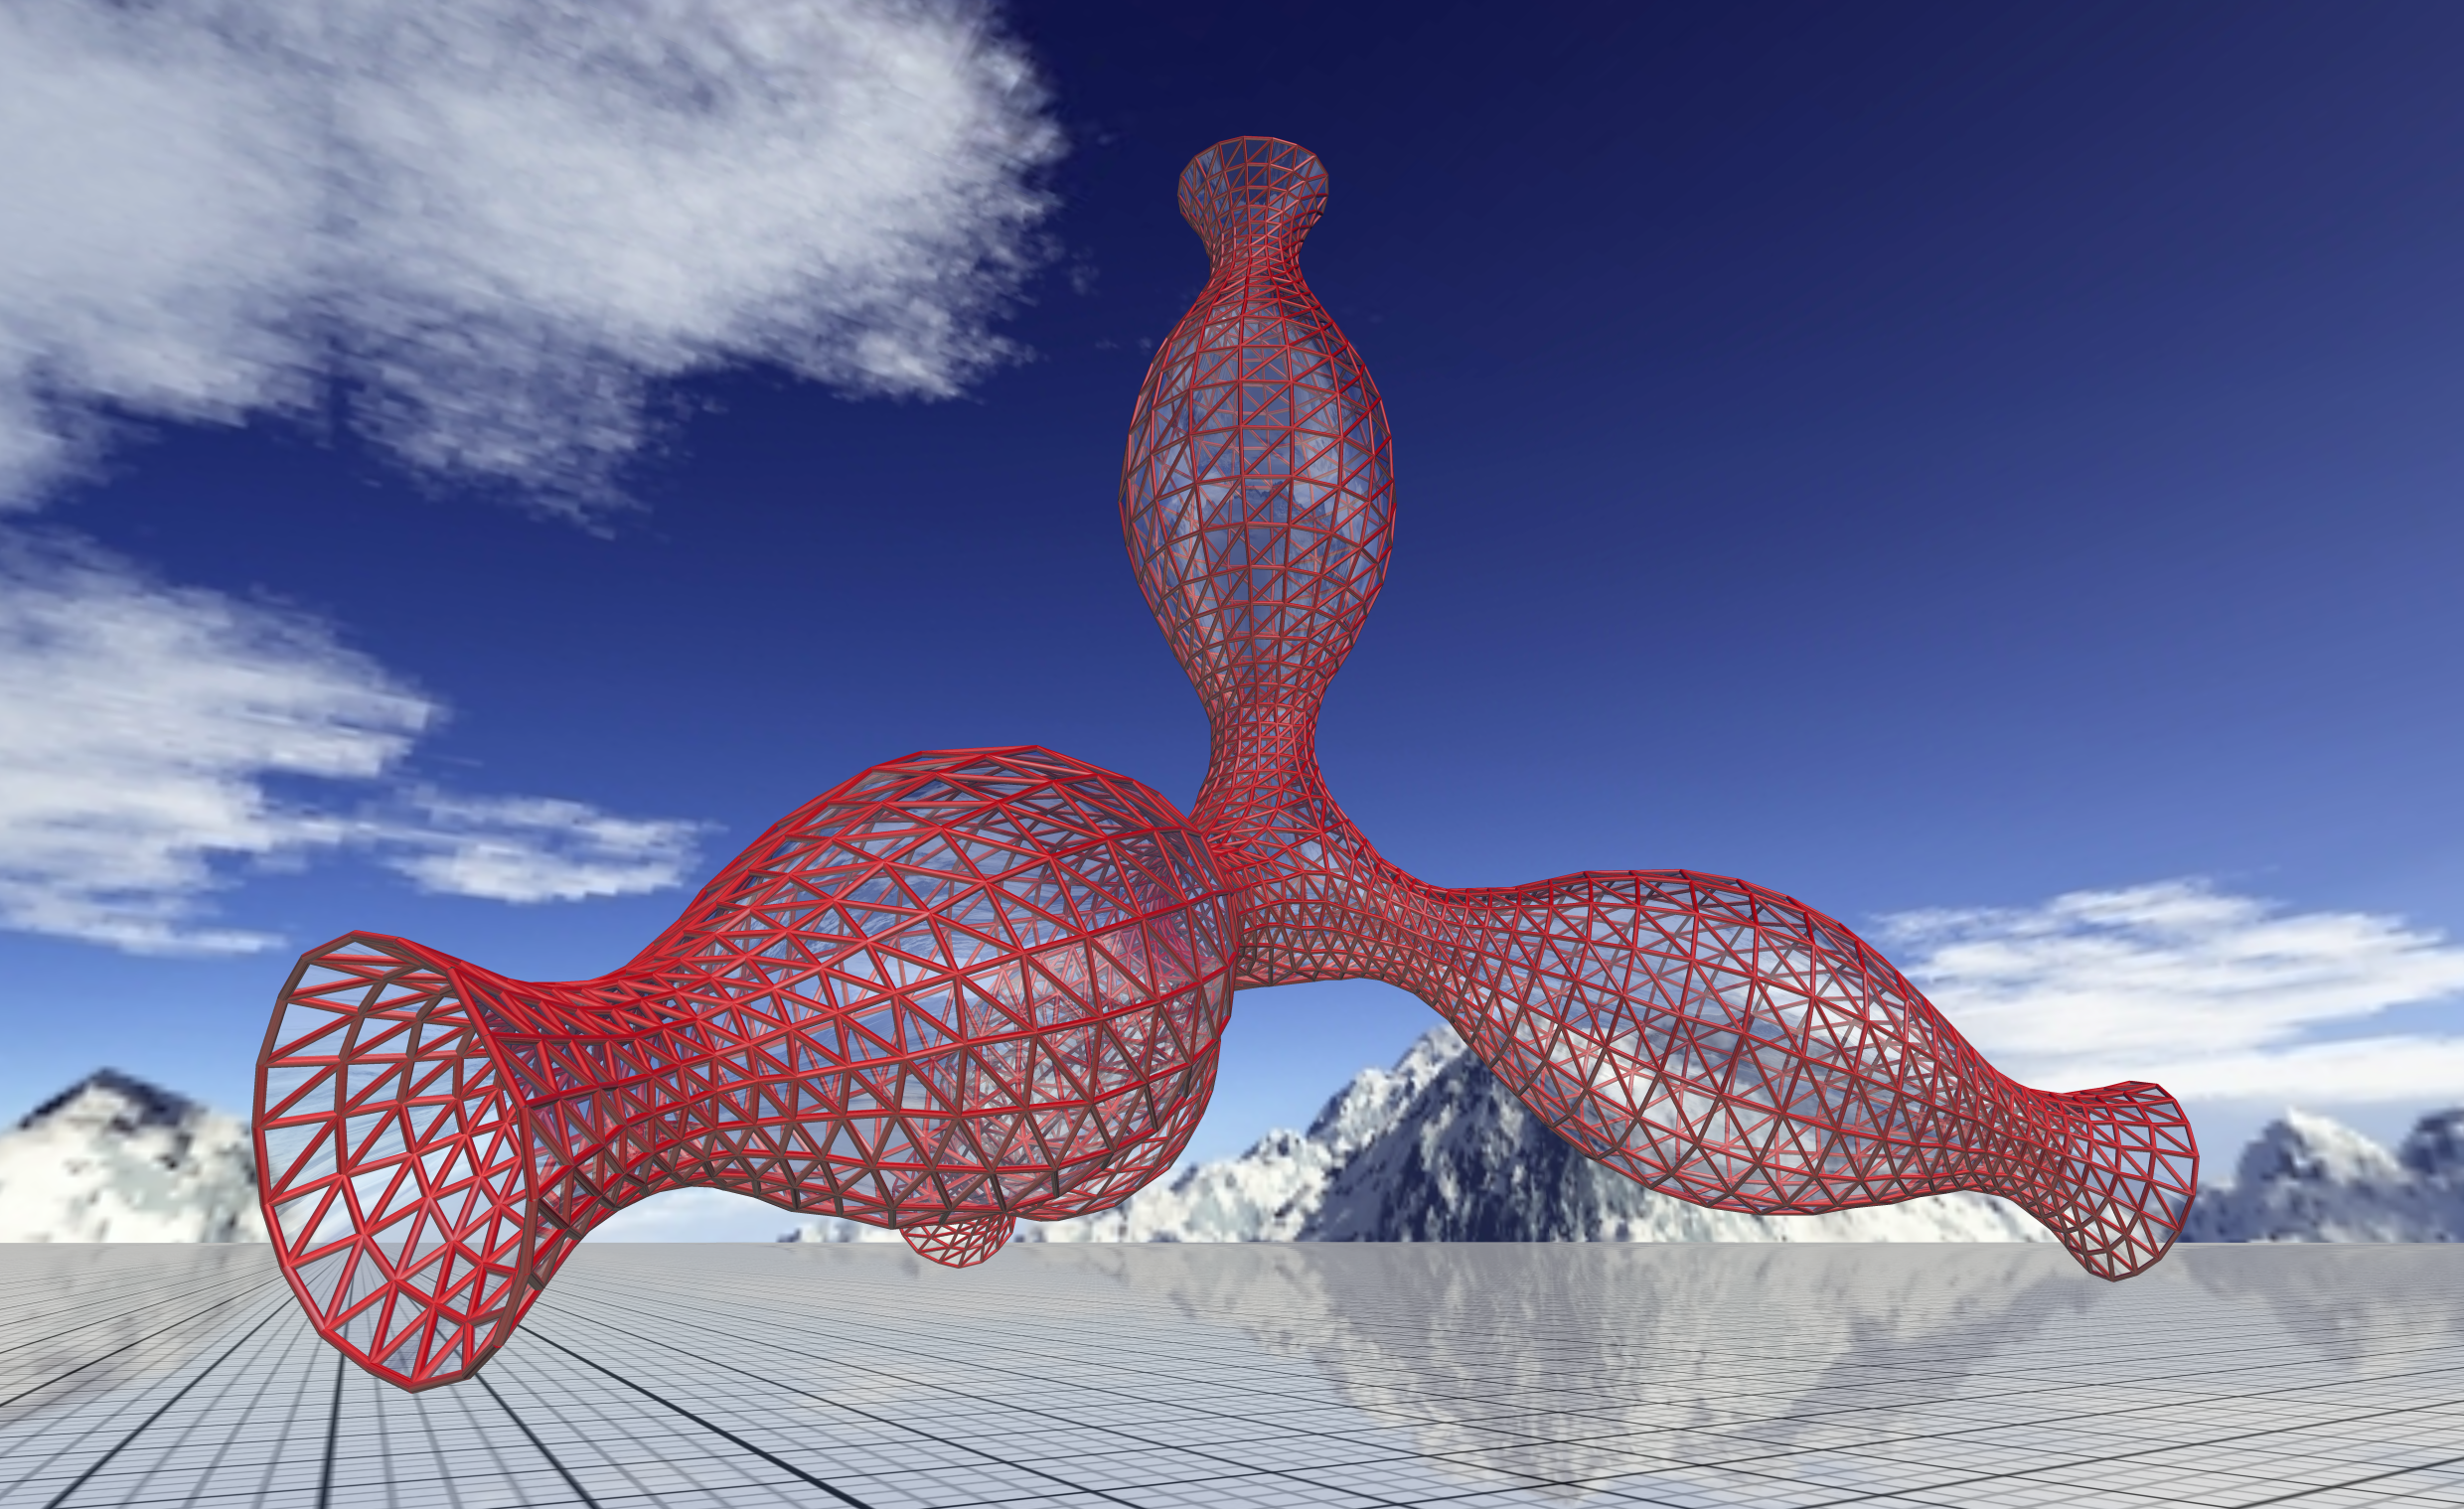
\includegraphics[width=1\textwidth]{jReality.png}
	\end{column}%
\end{columns}
\end{frame}


\begin{frame}[t]{Architektur}
\vspace{1.5cm}
	\begin{itemize}
		\item Eventbasierte Stern-Architektur \pause
		\item Lose Kopplung zwischen den Komponenten \pause
		\item Asynchrone Brücken zwischen Java und Polymke \pause
		\item Berechnungsanfragen als Perl-Programme \pause
		\item Symmetriegruppen als einzelne Klassen
	\end{itemize}
\vspace{1cm}
\only<5->{\emph{Siehe folgendes Bild}}
\end{frame}

\begin{frame}{Architektur}
\includegraphics[width=1\textwidth]{architecture.png}
\end{frame}

\begin{frame}{Demo}
\huge{Siehe: Live-Demo}
\end{frame}

\begin{frame}{Zusammenfassung der Funktionen}
	\begin{itemize}
		\item Auswahl 3D/4D \pause
		\item Symmetriegruppen: Tetraeder, Oktaeder \& Ikosaeder \pause
		\item Punktwahl im Raum, Eingabe oder zufällig \pause
		\item Darstellung des Fundamentalbereichs \pause
		\item Darstellung der Punktgruppe als Schlegeldiagramm \pause
		\item Logbuch 	
	\end{itemize}
\end{frame}

\begin{frame}{Lesson Learned}
	\begin{itemize}
		\item Für Projekt und Teilnehmeranzahl gutes Prozessmodell \pause
		\item Wöchentliches Meeting sinnvoll \pause
		\item Protokoll hilfreich zur Erinnerung und Fokussierung der Besprechung (Spline-Pad) \pause
		\item Persönliche Kommunikation notwendig \pause
		\item Meist guter Einsatz von Git \pause
		\item Verwendung von Fremdsoftware aufwendig \pause
		\item Softwareprojekte als Blockkurs sind angenehmer \pause
	\end{itemize}
\end{frame}

\begin{frame}{Ausblick}
\begin{itemize}
	\item Symmetriegruppen aus Erzeugern generieren
	\item GUI verschönern
	%\item Schnittstelle um Polyeder im 3D-Drucker ausdrucken zu können
	\item Logbucheintragstufe einstellen
	\item Parallelisierung der Anfragen an Polymake
\end{itemize}
\end{frame}


\begin{frame}[t]{Fragen}
\huge{Vielen Dank für die Aufmerksamkeit!} \\
\vspace{1cm}
\only<2->{\huge{Fragen?}
\includegraphics[height=0.75\textheight]{lehrer_laempel.png}
}
\end{frame}
\end{document}
